\chapter{Introduction}
\label{chapter:introduction}
\lhead{Chapter 1. \emph{Introduction}}

\section{Motivation and Framing}
%Here is an abbreviation: artificial intelligence (AI)\label{label_ai}
Approximately 90\% of the global trade being carried by the international shipping industry, turning the Ocean vital for the Worlds economy.
Nowadays there are approximately 50,000 merchant ships trading internationally, and with the current demand this number tends to increase~\cite{ICS}.

Although this efficient way of transportation creates a huge opportunity for illicit activities and organized crime.
There are several threats that prevail in the maritime domain(i.e. piracy, trafficking of drugs, illegal immigration, arms proliferation, illegal fishing etc). The definition of maritime safety is complex, but it's acknowledged as a transnational task~\cite{Bueger2015}.

Nowadays tracking people and objects in a geographical space has become ubiquitous.
Automatic Identification System (AIS)\label{label_AIS} is an automated tracking system, that broadcasts information thought VHF mobile maritime band assisting vessels in navigation. 
Imposed by the IMO (International Maritime Organization)\label{label_IMO} every SOLAS
(Safety of Life at Sea) \label{label_SOLAS} vessel must be equipped with an AIS device.

Autonomously broadcast AIS messages contain kinematic information (including ship location, speed, heading, rate of turn, destination and estimated arrival time) and static information (including ship name, ship MMSI ID, ship type, ship size and current time). AIS messages can be transformed into useful information for maritime traffic manipulations (e.g. vessel path prediction and collision avoidance). Therefore the AIS messages play a central role in the future autonomous maritime navigation systems~\cite{Mao2016}.

The introduction of AIS in the maritime domain increased the volume of Vessel trajectory data exponentially, making human analysis and evaluation of this data extremely inefficient. Therefore, new effective ways of automatically mining this data show a great contribution for the future of nautical surveillance. However mining maritime trajectory data present several challenges: 

First, maritime trajectory data possess the data uncertainty typical of moving object trajectories.
Geo-referenced locations of trajectory positioned by location sensing techniques may be collected with spatial uncertainty due to computational error and signal loss or degradation associated with the positioning device. Temporal uncertainty can be generated by different sampling rates and temporal lengths~\cite{Lee}. Secondly, maritime traffic is not constraint to roads; Vessels are free to navigate in open waters 
as long maritime laws are respected, therefore the complexity of anomaly detection increases drastically.

Nevertheless, to their advantage Vessels try to travel always in the most economic route, creating a behavioural baseline that is important for this work. Although a strong definition of anomalous behaviour is needed and it can be sub-divided in two categories:

\begin{description}
\item[Kinematic behaviours] relate to the motion of ships including the routes taken and speed of travel.
\item [AIS transmission behaviors] include the switching on or off of AIS systems and changing the vessels name or other details. Other behaviors such as changes in crew members, or ship registration details could also be categorized ~\cite{Lane2010}.
%On this work the focus will be on anomalous behavior that can be described using AIS data.
\end{description}

In chapter ~\ref{chapter:literatureReview} a solid state of the art is presented, with the emphases on methods and algorithms that mine trajectories data, in order to achieve a system that satisfies the main research question.


\section{Research Methodology}
The scope of the course 'Introduction to Research in Engineering', presents the students with a research methodology.

DSRM, is an outcome based research methodology in specific guidelines for evaluation and iteration over research projects are presented.

DSRM is a research topic in various fields, presenting specific methods, for different areas of research. 

Not only for the scope of the course, but also for Literature Review presented in Chapter~\ref{chapter:literatureReview}. A similar research methodology, as the one presented in ~\cite{Peffers2007}, was followed.
The authors present a process model consisting of the following six activities in a nominal sequence as presented in Figure~\ref{fig:DSRMPeffers}.

\begin{figure}[H]
	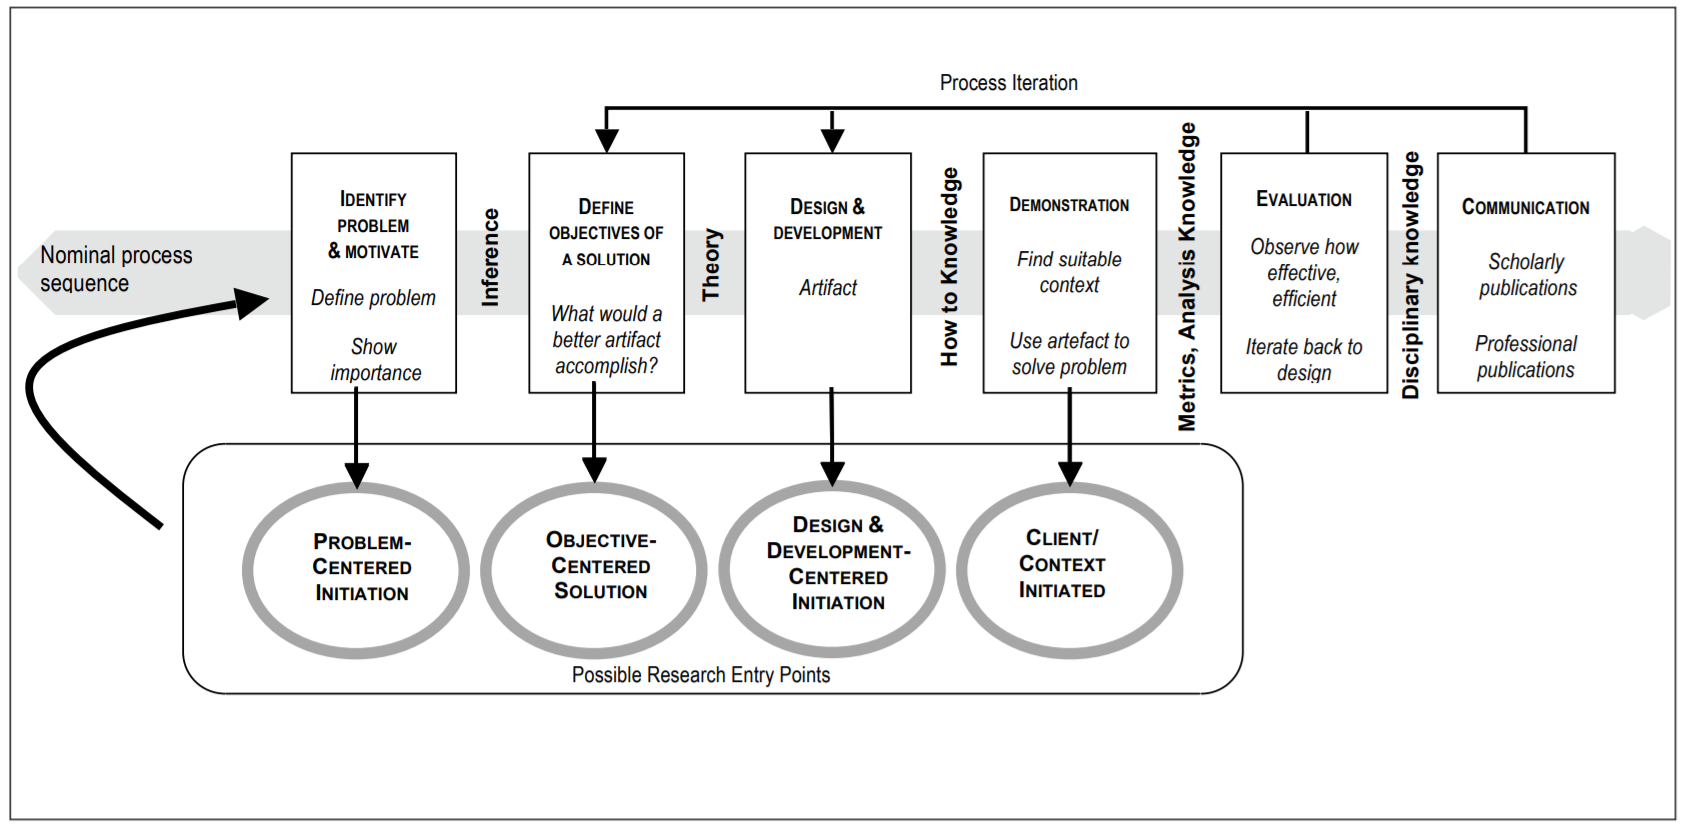
\includegraphics[width=\linewidth]{figures/DSRMPeffers.PNG}
    \caption{Design Science Research Methodology, ~\cite{Peffers2007}}
    \label{fig:DSRMPeffers}
\end{figure}

\subsection{Problem identification and motivation:} 
The process of identifying vessels with an abnormal behaviour, is a complex task. This is mainly because in vessels, abnormal behaviour can be caused by numerous different causes.
  
The authors ~\cite{Laxhammar2008} define Anomaly Detection (AD) as "a method for separating an often in-homogeneous and hard characterized minority of data from a more regular majority of data, by studying and characterizing the majority, so that data in the minority appears as deviations from the patterns found in the majority". 

The main focus of this work is the research and develop of methods that represent vessel motion data, in ways that anomalies can be found.

The MARISA project involves 22 organizations completely motivated to fulfil the overarching objective. 

With the current needs of an more comprehensive approach at the European seas, new and more efficient methods that promote the information exchange between European Union countries, optimizing the European maritime area surveillance and its maritime borders are a current need.

The MARISA project is funded under an H2020, which is an financial instrument that promotes innovation through the European Union.

\subsection{Define the objectives for a solution:}
The research problem is defined accordingly with the MARISA project, which can be defined as: 

~\textit{How to create a system that fuses Data from different sources, capitalizing on the large amount of unexploited maritime data, while autonomously identifying Anomalous Vessel Behaviour.}  

Due to the complexity of this main question, it's important to divide it into smaller questions:

\begin{itemize}
\item Which sources are the most viable to gather spatial data from Vessels,
turning it into a sound Data-Set?
\item Which techniques can transform Spatial Data into Sequential Data, thus creating Vessel trajectories?
\item Can previous Algorithms mine trajectory data from AIS sources, finding anomalies?
\end{itemize}

\subsection{Design and development:} In order to achieve the proposed goals, and simultaneous contribute to the MARISA project the two following objectives were created, in Design Science Research this objectives are described as artifacts:

\begin{itemize}
\item \textbf{Data-Set} A solid Data-Set must be gathered and cleaned. Through the MARISA project, the process of obtaining a Data-Set can be prolonged.Thus ways of obtain AIS Data-Sets free of cost must be researched.

\item \textbf{Route Definition} Numerous methods of vessel route definition, are presented in ~\ref{chapter:literatureReview}.
Although, at this moment a method was chosen that represents the route as a whole. Therefore no information is lost, a detailed description of the latter is presented in ~\ref{section: Trajectory Analysis}.
\end{itemize}

\subsection{Demonstration}https://v2.overleaf.com/project/5b094c27dd648c7b207643b4
While the first artifact is a necessity for future work, is on this data-set that future work will be developed. At this moment I'm using a data-set, from the North America region that has 3.3 million AIS messages, from various vessels.
All the MARISA requirements, will in a initial phase, be developed on this data-set.
\subsection{Evaluation}
The evaluation of the future artefacts, will be firstly conducted by INOV, and after by MARISA partners.
Performance assessment of the artefacts, will be considered after the first implementation is concluded.

\subsection{Communication} 
The research is being conducted for the fulfilment of my masters, therefore a dissertation will be presented for the final evaluation. There is the possibility of submitting future articles for publishing, this possibility depends on the MARISA project.
